% !Mode:: "TeX:UTF-8"
% VL 4, gebaut aus part-lernen/06-logistische-regression.md
% (Dialogmuster und Zeiten: transcripts/vl04-logistische-regression-2025/notiz.md).
% !Mode:: "TeX:UTF-8"
\newcommand{\thepage}{} % to silence a hyperref warning about pdfpagelabels
\RequirePackage[]{silence}
\WarningsOff[hyperref]
\PassOptionsToPackage{log-declarations=false}{xparse}
%\RequirePackage[l2tabu, orthodox]{nag}
\RequirePackage{luatex85} % to make \pdf...= commands work with LuaTeX
\documentclass[aspectratio=169,t]{beamer}
\usepackage{ifthen}
\usepackage[T1]{fontenc}
\usepackage{iftex}
\ifLuaTeX
 \usepackage{fontspec}
 \setmainfont[Ligatures=TeX]{Source Sans Pro}
\else
 \usepackage[utf8]{inputenc}
\fi
\usepackage{german}
\usepackage{newunicodechar}
\newunicodechar{€}{\texteuro}
\newunicodechar{ß}{\ss}
\renewcommand{\SS}{\iffontchar\font"1E9E \symbol{"1E9E}\else SS\fi}
\usepackage{ellipsis}
\usepackage{microtype}
\usepackage{listings}
\usepackage{sourcecodepro}
\lstset{language=Python, basicstyle=\ttfamily}
\usepackage{amsfonts}
\usepackage{amssymb}
\usepackage{amsthm}
\usepackage{fancyhdr}
\usepackage{graphicx}

\newtheorem{proposition}[theorem]{Proposition}

\DeclareMathOperator*{\argmax}{argmax}
\DeclareMathOperator{\supp}{supp}
\newcommand{\E}{\ensuremath{\mathbb{E}}}
\newcommand{\V}{\ensuremath{\mathbb{V}}}

\setbeamercolor{emph}{fg=purple}
\renewcommand<>{\emph}[1]{%
  {\usebeamercolor[fg]{emph}\only#2{\itshape}#1}%
}



\hypersetup{draft=false,colorlinks=false,pdfpagemode=UseOutlines,plainpages=false,
            breaklinks=true,bookmarksnumbered=true,pdfborder=0 0 0,
            pdftitle={Einführung in Deep Learning WiSe 2026/27 HHU},
            pdfauthor={Konrad Voelkel},
            pdfsubject={data science}}

%\documentclass[aspectratio=169,t]{beamer}
\usetheme{hhubeamer} % put the hhu-beamer-theme in /usr/share/texmf/tex/latex/beamer/themes/

% -------------------- Code listings config --------------------
% Define custom colors for syntax highlighting
\definecolor{codegreen}{rgb}{0,0.6,0}
\definecolor{codegray}{rgb}{0.5,0.5,0.5}
\definecolor{codepurple}{rgb}{0.58,0,0.82}
\definecolor{backcolour}{rgb}{0.96,0.96,0.94} % Very light gray/beige
% Configure the listings package
\lstset{
    language=Python,
    backgroundcolor=\color{backcolour},   
    commentstyle=\color{codegreen}\itshape,
    keywordstyle=\color{blue}\bfseries,
    numberstyle=\tiny\color{codegray},
    stringstyle=\color{codepurple},
    basicstyle=\ttfamily\footnotesize, % Use a monospaced font
    breakatwhitespace=false,         
    breaklines=true,      
             % Enable automatic line breaking
    captionpos=b,                      % Caption at the bottom
    keepspaces=true,                 
    numbers=left,                      % Line numbers on the left
    numbersep=10pt,                    % Distance of line numbers from the code
    showspaces=false,                
    showstringspaces=false,            % Don't show weird underscores in strings
    showtabs=false,                  
    tabsize=4,
    frame=single,                      % Add a subtle border around the code
    rulecolor=\color{black!20},        % Border color
  }

\event[]{}
\author[Wintersemester 2026/27]{Dr. Konrad Völkel, Wintersemester 2026/27}

%\title{Data Science, VL 1}
%\date{16.04.2026}


%%% Local Variables:
%%% mode: latex
%%% TeX-master: t
%%% End:


% Fassung mit Dozentennotizen (zweiter Schirm): die nächste Zeile einkommentieren.
% \setbeameroption{show notes on second screen=right}

\graphicspath{{../images/}}

\title[Logistische Regression (VL 4)]{Logistische Regression\\\large Einführung in Deep Learning, VL 4}
\date{04.11.2026}

\begin{document}

\begin{frame}
  \titlepage

  \note{\textbf{Ablauf, 90 Minuten} (2025: 60 Min. Konzept, 27 Min. Code, 3 Min. Übungstipps):\\[2pt]
    \begin{tabular}{@{}rll@{}}
      0--8   & Folien 2--4   & Lineare Regression zur Klassifikation, S-Form basteln\\
      8--20  & Folien 5--7   & Wahrscheinlichkeit, Odds, die Skala\\
      20--30 & Folien 8--9   & Logit, Entropie\\
      30--42 & Folien 10--12 & Sigmoid, Symmetrie, Ableitung\\
      42--50 & Folien 13--14 & Sigmoid und Logit sind invers -- die Interpretation\\
      50--56 & Folie 15      & Logistische Regression, Definition\\
      56--72 & Folien 16--18 & \textbf{PyTorch: die Trainingsschleife}\\
      72--82 & Folien 19--20 & Softmax, wann er passt\\
      82--87 & Folie 21      & Numerik: warum der Loss \texttt{nan} wird\\
      87--90 & Folie 22      & Übungsblatt\\
    \end{tabular}\\[4pt]
    2025 war der Stoff nach 75 Minuten durch und der Rest wurde Vorgriff auf VL 5.
    Besser: die Trainingsschleife langsamer durchgehen, sie ist die Blaupause für
    alles Weitere.}
\end{frame}

\begin{frame}
  \frametitle{Wo wir stehen}

  \begin{center}
    \Large
    Verallgemeinertes Perzeptron: $f(x) = \tau(w \cdot x)$\\[16pt]
    Heute: $\tau = \sigma$ -- und warum das eine \emph{Wahrscheinlichkeit} ist.
  \end{center}

  \note{Erst basteln wir eine S-Kurve aus dem $\tanh$ und haben keine Interpretation dafür.
    Dann bauen wir dieselbe Kurve von der Wahrscheinlichkeitsrechnung her auf -- und die
    Interpretation fällt von selbst ab. Das ist die Dramaturgie der Sitzung.}
\end{frame}

% ------------------------------------------------------------------ lineare Regression
\begin{frame}
  \frametitle{Lineare Regression zur Klassifikation}

  \begin{center}
    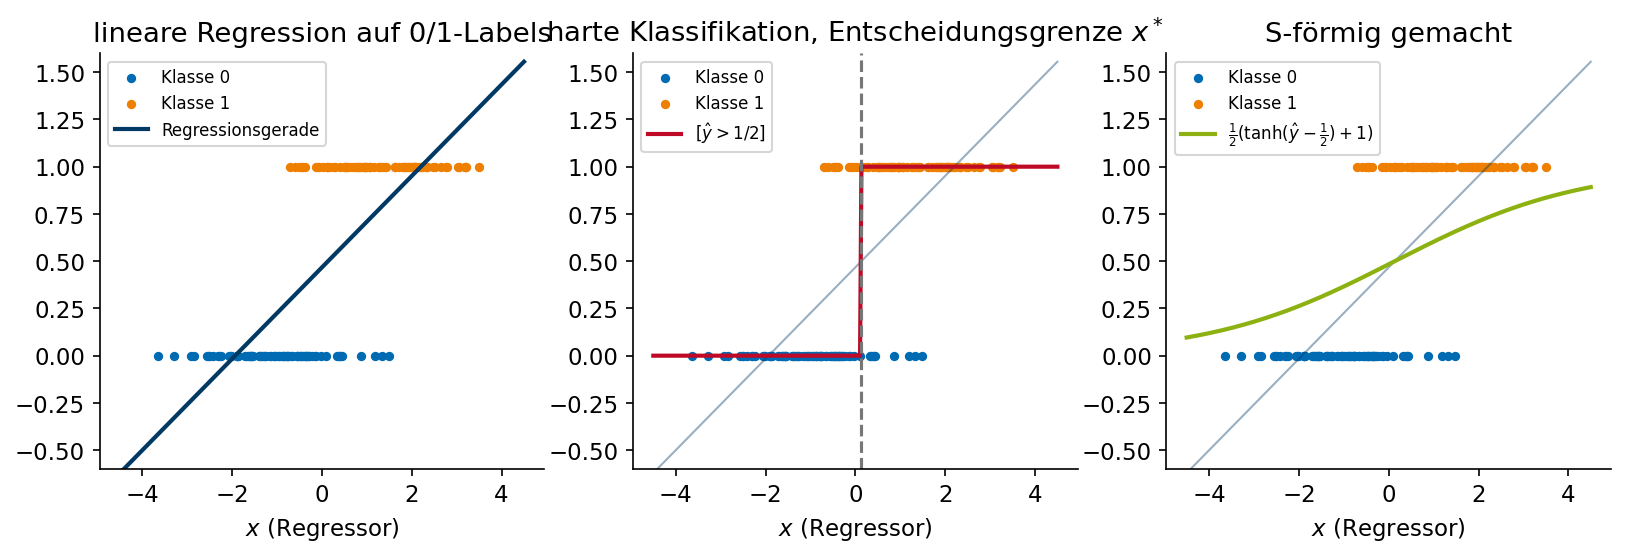
\includegraphics[width=0.85\textwidth]{vl03-linreg-classification-1d.png}
  \end{center}

  \note{Schrittweise vorlesen: Punkte liegen auf $y = 0$ und $y = 1$; die Regressionsgerade
    nimmt Werte in ganz $\mathbb{R}$ an; harte Klassifikation bei $\hat{y} > \frac12$;
    die Entscheidungsgrenze ist der Punkt $x^*$ mit $wx^* + b = \frac12$.
    Rechts schon die $\tanh$-Variante -- darauf kommen wir gleich.}
\end{frame}

\begin{frame}
  \frametitle{Zweidimensional}

  \begin{center}
    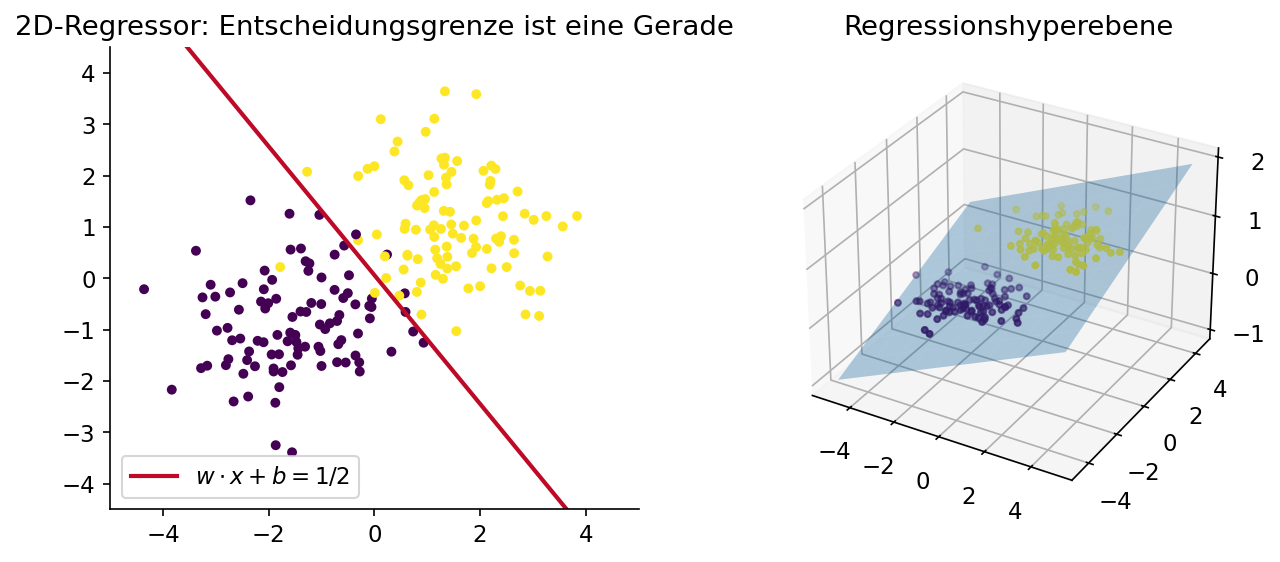
\includegraphics[width=0.8\textwidth]{vl03-linreg-classification-2d.png}
  \end{center}

  \note{Aus der Geraden wird eine Ebene über der $(x_1,x_2)$-Ebene, und die
    Entscheidungsgrenze $\{w \cdot x + b = \frac12\}$ ist wieder eine Gerade -- genau wie
    beim Perzeptron. Die Brücke zur letzten Woche hier ausdrücklich schlagen.}
\end{frame}

\begin{frame}
  \frametitle{S-Förmigkeit basteln}

  \begin{center}
    \Large $\tfrac12\left(\tanh(\hat{y}) + 1\right)$
  \end{center}

  \bigskip
  \begin{center}
    Glatt, zwischen 0 und 1 -- aber \emph{warum} sollte das eine Wahrscheinlichkeit sein?
  \end{center}

  \note{Die Sprungfunktion ist unbefriedigend: nicht differenzierbar, und sie verrät nicht,
    wie sicher die Entscheidung ist.
    Eine abgelehnte Alternative, die 2025 aus dem Hörsaal kam: einfach $2p - 1$ -- geht
    auch, hat aber dieselbe fehlende Interpretation.
    Die offene Frage bleibt bewusst stehen; jetzt Themenwechsel zur Wahrscheinlichkeitsrechnung.}
\end{frame}

% ------------------------------------------------------------------ Odds
\begin{frame}
  \frametitle{Wahrscheinlichkeit und Chancen}

  \begin{center}
    \Large
    $P(D = 6) = \tfrac16$\\[14pt]
    $\operatorname{odds}(D = 6) = \dfrac{1/6}{5/6} = \dfrac15$
  \end{center}

  \bigskip
  \begin{center}
    $\operatorname{odds}(p) = \dfrac{p}{1-p}$, \qquad $p = \dfrac{\operatorname{odds}}{1+\operatorname{odds}}$
  \end{center}

  \note{Odds kommen aus Pferdewetten -- das ist die Herkunft und hilft der Intuition:
    $1{:}5$ liest sich als „einer gegen fünf“.
    Frage in den Raum: Was sind die Odds für eine \emph{Nicht}-6? Antwort $5$, nicht
    $\frac45$ -- das ist der Punkt für die nächste Folie.}
\end{frame}

\begin{frame}
  \frametitle{Die Skala für Odds ist schief}

  \begin{center}
    \Large
    $p < \tfrac12 \;\Rightarrow\; \operatorname{odds} \in [0,1)$\\[10pt]
    $p > \tfrac12 \;\Rightarrow\; \operatorname{odds} \in (1,\infty)$
  \end{center}

  \bigskip
  \begin{center}
    Erfolg und Misserfolg sind symmetrisch -- die Skala ist es nicht.
  \end{center}

  \note{Beschränkt auf der einen, unbeschränkt auf der anderen Seite. Die Odds für eine 6
    sind $\frac15$, die für eine Nicht-6 sind $5$.
    Frage: Wie repariert man das? Antwort abwarten -- Logarithmieren.}
\end{frame}

\begin{frame}
  \frametitle{Logarithmieren rettet die Symmetrie}

  \begin{center}
    \Huge $\operatorname{logit}(p) = \ln \dfrac{p}{1-p}$
  \end{center}

  \bigskip
  \begin{center}
    $\ln(1{:}5) = -\ln(5{:}1)$, \qquad Werte in $(-\infty, +\infty)$
  \end{center}

  \note{Logit = \emph{logistic unit}, eine künstliche Einheit wie das Bit.
    Schon mal gesehen? Im Data-Science-Skript: Informationsgehalt $-\log p$, Entropie als
    erwartete Überraschung. Der Logarithmus steht dort aus demselben Grund: unabhängige
    Ereignisse multiplizieren Wahrscheinlichkeiten, $\log$ macht daraus eine Summe.
    Münzwurf 1 bit, eine 6 beim Würfeln $\log_2 6 \approx 2{,}58$ bit, zusammen 3,58 bit.}
\end{frame}

\begin{frame}
  \frametitle{Entropie und Logit}

  \begin{center}
    \Large
    $H(p) = -p\ln p - (1-p)\ln(1-p)$\\[16pt]
    $H'(p) = -\operatorname{logit}(p)$
  \end{center}

  \note{Interpretation: Beim Erhöhen von $p$ ist die Abnahme an Informationsgewinn durch
    $\operatorname{logit}(p)$ gegeben. Entropie misst man in bit ($\log_2$) oder nat ($\ln$),
    die Ableitung in Logit. $H(0{,}5) = 1$ bit $= 0{,}69$ nat.
    \textbf{Achtung, Stolperstelle aus 2025:} Wenn hier ein Plot mit beiden Kurven kommt --
    die Ableitung ist $-\operatorname{logit}$, also an der $x$-Achse gespiegelt. 2025 kam
    aus dem Hörsaal genau diese Korrektur.}
\end{frame}

% ------------------------------------------------------------------ Sigmoid
\begin{frame}
  \frametitle{Die logistische Funktion}

  \begin{center}
    \Large
    $S(x; M, k, \mu) = \dfrac{M}{1 + e^{-k(x-\mu)}}$\\[16pt]
    $\sigma(x) = \dfrac{1}{1+e^{-x}}$
  \end{center}

  \note{$M$ ist die obere Asymptote, $k$ die Steilheit, $\mu$ die Lage des Wendepunkts.
    Bei $\sigma(w \cdot x + b)$ übernimmt $\|w\|$ die Rolle von $k$ -- das ist der
    Rückbezug auf VL 2: Die Länge von $w$ bestimmt, wie schnell die Wahrscheinlichkeit
    mit dem Abstand zur Grenze wächst.
    Sigma $\approx$ S, Sigmoid $\approx$ S-förmig.}
\end{frame}

\begin{frame}
  \frametitle{Sigmoid, tanh, Ableitung}

  \begin{center}
    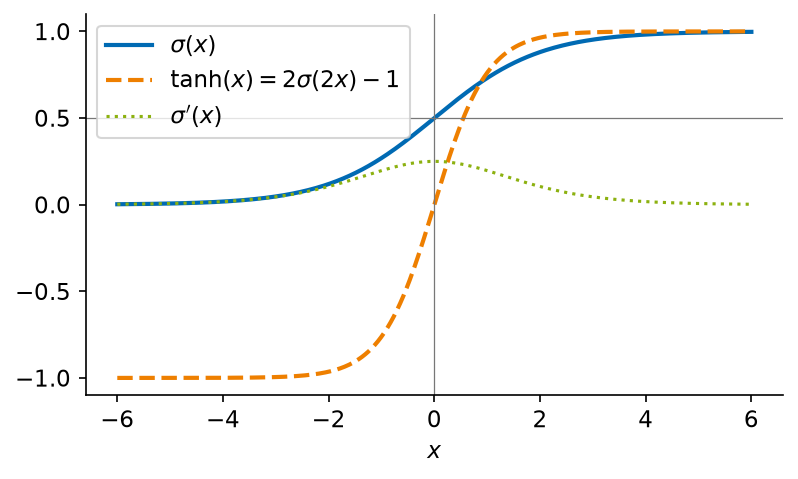
\includegraphics[width=0.62\textwidth]{vl04-sigmoid.png}
  \end{center}

  \note{$\tanh(x) = 2\sigma(2x) - 1$ -- nur ein umskaliertes Sigmoid, das rechnet man in
    zwei Zeilen nach.
    $\sigma' = \sigma(1-\sigma)$ mit Maximum $\frac14$ bei 0. Bemerkenswert: Die Ableitung
    lässt sich aus dem \emph{Funktionswert} berechnen, ohne $e^{-x}$ noch einmal
    auszuwerten -- das ist beim Training praktisch. Der Beweis mit der Quotientenregel
    ist eine Übungsaufgabe.}
\end{frame}

\begin{frame}
  \frametitle{Symmetrie}

  \begin{center}
    \Huge $\sigma(-x) = 1 - \sigma(x)$
  \end{center}

  \bigskip
  \begin{center}
    Punktsymmetrisch um $(0, \tfrac12)$.
  \end{center}

  \note{Die Rechnung ist kurz genug für die Tafel: mit $e^{-x}$ erweitern, dann sieht man
    es. Diese Identität brauchen wir bei der Kreuzentropie wieder.}
\end{frame}

\begin{frame}
  \frametitle{Sigmoid und Logit sind invers}

  \begin{center}
    \Large
    $\sigma \circ \operatorname{logit} = \operatorname{id}_{(0,1)}$\\[12pt]
    $\operatorname{logit} \circ \sigma = \operatorname{id}_{\mathbb{R}}$
  \end{center}

  \note{Beide Rechnungen stehen im Skript und sind je drei Zeilen; eine davon an der Tafel
    vorrechnen, die andere als Übung lassen.
    Deshalb heißt $\sigma$ auch \emph{expit} -- der Name ist veraltet, aber er erklärt,
    was gemeint ist.}
\end{frame}

\begin{frame}
  \frametitle{Und damit die Interpretation}

  \begin{center}
    \Large
    Jede Zahl $x \in \mathbb{R}$ darf man als \emph{Logit} lesen.\\[16pt]
    $\sigma(x)$ ist dann die Wahrscheinlichkeit,\\
    zu der $x$ der Logit-Wert ist.
  \end{center}

  \note{Das ist die Antwort auf die Frage von Folie 4, und die Take-Home-Message der
    Sitzung. Eine Zahl zwischen 0 und 1 ist eine Wahrscheinlichkeit, \emph{wenn} die
    Eingabe ein Logit war -- nicht einfach, weil sie zwischen 0 und 1 liegt.}
\end{frame}

\begin{frame}
  \frametitle{Logistische Regression}

  \begin{center}
    \Huge $f(x) = \sigma(w \cdot x + b) = P(Y = 1 \mid X = x)$
  \end{center}

  \bigskip
  \begin{center}
    \normalsize In Scikit-Learn: \texttt{predict\_proba} gegen \texttt{predict}.
  \end{center}

  \note{Das verallgemeinerte Perzeptron mit $\tau = \sigma$.
    Entscheidung für Klasse 1, wenn $\sigma(\hat{y}) > \frac12$ -- und weil $\sigma$
    monoton ist mit $\sigma(0) = \frac12$, ist das dasselbe wie $\hat{y} > 0$.
    \texttt{predict} ist also \texttt{predict\_proba} mit Schwelle.}
\end{frame}

% ------------------------------------------------------------------ PyTorch
\begin{frame}[fragile]
  \frametitle{Lineare Regression in PyTorch}

  \begin{lstlisting}
class LinearRegression(nn.Module):
    def __init__(self, input_dim, output_dim):
        super().__init__()
        self.linear = nn.Linear(input_dim, output_dim)

    def forward(self, x):
        return self.linear(x)
  \end{lstlisting}

  \note{Ein Modell ist eine Unterklasse von \texttt{nn.Module}: im Konstruktor die
    Bausteine mit Parametern, in \texttt{forward} die Inferenz. \texttt{nn.Linear} ist
    $x \mapsto Wx + b$, der Bias ist eingebaut.
    2025 kam der Einwurf, dass \texttt{forward} nirgends direkt aufgerufen wird. Antwort:
    Der Aufruf des Modellobjekts ist Syntactic Sugar für \texttt{forward} -- und deshalb
    \emph{muss} die Methode so heißen.}
\end{frame}

\begin{frame}[fragile]
  \frametitle{Die Trainingsschleife}

  \begin{lstlisting}
for epoch in range(number_of_epochs):
    optimizer.zero_grad()          # Gradienten auf null
    outputs = model(inputs)        # Vorwaertsrechnung
    loss = criterion(outputs, labels)
    loss.backward()                # Gradienten rueckwaerts
    optimizer.step()               # Parameter anpassen
  \end{lstlisting}

  \bigskip
  \begin{center}
    Diese fünf Zeilen begleiten uns durch das ganze Semester.
  \end{center}

  \note{\textbf{Das ist die Blaupause} -- hier langsam machen, jede Zeile benennen.
    Was \texttt{criterion} (MSE) und \texttt{optimizer} (SGD, Lernrate 0,01) genau tun,
    klären VL 5 und VL 6. Heute reicht: es gibt beides, und es sind austauschbare Teile.
    Nebenbei erklären, falls gefragt: \texttt{reshape(-1, 1)}, weil PyTorch eine
    Batch-Achse erwartet (VL 3!), und \texttt{float32}, weil das der Standard-dtype ist.}
\end{frame}

\begin{frame}[fragile]
  \frametitle{Und jetzt logistisch}

  \begin{lstlisting}
    def forward(self, x):
        return torch.sigmoid(self.linear(x))   # <---

criterion = nn.BCELoss()                       # <---
  \end{lstlisting}

  \begin{center}
    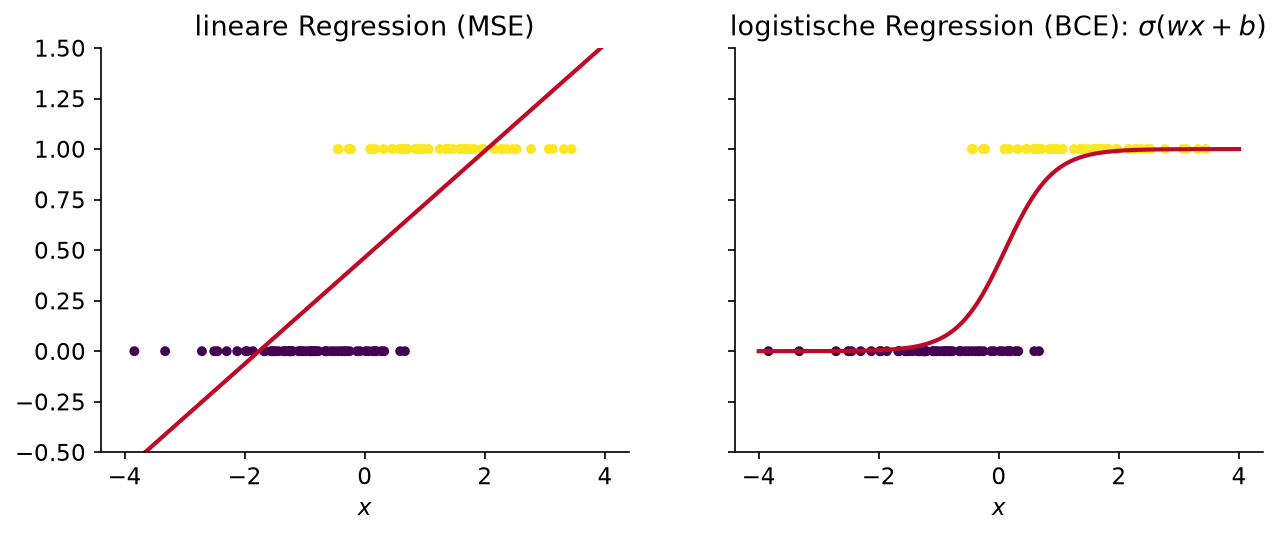
\includegraphics[width=0.46\textwidth]{vl04-lin-vs-log-regression.png}
  \end{center}

  \note{Zwei Zeilen Unterschied -- das ist die Pointe. Sigmoid im \texttt{forward},
    BCE statt MSE als Loss.
    Das Bild zeigt dieselben 0/1-Daten, einmal mit MSE, einmal mit BCE gefittet.
    Warum BCE und nicht MSE, kommt in VL 5. Wer jetzt schon fragt: MSE auf 0/1-Daten
    zählt im Grunde Fehlklassifikationen und straft sichere Fehler zu milde.}
\end{frame}

% ------------------------------------------------------------------ Softmax
\begin{frame}
  \frametitle{Mehr als zwei Klassen: Softmax}

  \begin{center}
    \Huge $\operatorname{sm}(v)_j = \dfrac{e^{v_j}}{\sum_k e^{v_k}}$
  \end{center}

  \bigskip
  \begin{center}
    \normalsize Kein Minus im Exponenten!
  \end{center}

  \note{\textbf{Achtung, hier ist 2025 Verwirrung entstanden:} Der Dozent glaubte, ein
    Minus vergessen zu haben. Es gehört keins hin -- die Formel ist so richtig. Das Minus
    in $\sigma(x) = 1/(1+e^{-x})$ entsteht erst beim Kürzen für $K = 2$.
    Probe: Alle Einträge positiv, Summe $\sum_j e^{v_j} / \sum_k e^{v_k} = 1$, also eine
    Wahrscheinlichkeitsverteilung -- ein Punkt im Wahrscheinlichkeitssimplex.
    Für $K = 2$ kommt genau das Sigmoid heraus, wobei nur die \emph{Differenz} der Logits
    zählt (Übungsaufgabe).}
\end{frame}

\begin{frame}
  \frametitle{Wann Softmax, wann nicht?}

  \begin{center}
    \Large
    Softmax, wenn $\operatorname{argmax}$ sinnvoll wäre.\\[16pt]
    \normalsize Katze \emph{oder} Hund \quad$\longrightarrow$\quad Softmax\\[8pt]
    mehrere Tags gleichzeitig \quad$\longrightarrow$\quad ein $\sigma$ pro Klasse
  \end{center}

  \note{Die Klassen müssen sich gegenseitig ausschließen, sonst ist die Normierung falsch.
    Beispiel aus 2025, das gut trug: Tier, Mensch, Hund, Katze -- das sind keine
    disjunkten Klassen, da ist Softmax die falsche Wahl.
    Wer will, kann hier die Brücke zu LLMs schlagen: Auch ChatGPT wählt am Ende aus einer
    Softmax-Verteilung, und was man statt \texttt{argmax} nimmt, ist eine eigene Frage
    (VL 12).}
\end{frame}

\begin{frame}
  \frametitle{Numerik: warum Ihr Loss \texttt{nan} wird}

  \begin{center}
    \Large
    In \texttt{float32} ist $e^{89} = \texttt{inf}$.\\[12pt]
    $\ln 0 = -\infty$, \quad $0 \cdot (-\infty) = \texttt{nan}$
  \end{center}

  \bigskip
  \begin{center}
    \normalsize \texttt{BCEWithLogitsLoss} und \texttt{CrossEntropyLoss} nehmen \emph{Logits}.
  \end{center}

  \note{Abhilfe ist immer dieselbe: nie erst $e^x$ und dann $\ln$, sondern beides
    algebraisch zusammenfassen. $\ln \sigma(z) = -\ln(1+e^{-z})$, für $z<0$ umgeschrieben
    als $z - \ln(1+e^{z})$. Beim Softmax das Maximum abziehen (log-sum-exp-Trick).
    Für das Übungsblatt ausdrücklich ansagen: Wenn der Loss \texttt{nan} wird, ist meistens das
    die Ursache -- nicht ein Fehler in der Trainingsschleife.}
\end{frame}

\begin{frame}
  \frametitle{Übungsblatt}

  \begin{itemize}\setlength{\itemsep}{8pt}
  \item Erst sehr einfache Testcases schreiben
  \item Den Loss beobachten: oben links anfangen, runter, unten bleiben
  \item Zum Debuggen \emph{ohne} Train-Test-Split arbeiten
  \end{itemize}

  \bigskip
  \begin{center}
    Nächste Woche: Woher kommt der Loss -- und wie wird er kleiner?
  \end{center}

  \note{Die Loss-Kurve ist die wichtigste Debug-Information: plotten, nicht nur die letzte
    Zahl angucken. Bei vielen Epochen lieber die ersten paar plotten.
    Warum ohne Split? Overfitting ist erst ein Problem, wenn überhaupt etwas gelernt
    wurde -- erst zum Laufen bringen, dann sauber machen.}
\end{frame}

\end{document}

%%% Local Variables:
%%% mode: latex
%%% TeX-master: t
%%% End:
